\graphicspath{{Chapter5/Figs/}}

\chapter{Future Research Agenda}
\label{chapter:future-research}

\section{Introduction}
To date, my research has focussed on using Gaussian processes (GPs) as building blocks for deep models, similar to neural network layers. In this vein, I have worked on (1) deep convolutional Gaussian processes that mimic the convolutional and layered architectures encountered in many contemporary deep learning models \citep{Dutordoir2020convolutional}, (2) conditional density estimation models which are similar to Variational Auto Encoders \citep{dutordoir2018cde,Salimbeni2019}, and more recently, (3) deep Gaussian processes that have basis functions that are similar to neural network activation functions \citep{dutordoir2021deep} (discussed at length in \cref{chapter:dnn-as-point-estimate-for-dgps}). I have packaged these advances in a software toolbox, called GPflux \citep{dutordoir2021gpflux}, which provides these GP layers through a neural network like interface. The main advantage of this approach is that straightforward application of Bayesian principles leads to sensible results, which is not necissarily the case for normal neural networks \citep{wenzel2020good}. The current state of research into using Gaussian processes as layers is that classification performance starting to be on-par with deep learning on simple datasets \citep{dutordoir2018cde}, but with better uncertainty quantification and automatic selection of hyperparameters working `out of the box'.

The primary focus of my previous research can be considered as `curve-fitting', i.e. finding the best function approximator when given examples of inputs and corresponding outputs. In this setting we can consider two regimes: (1) the function is complex but there is an abundance of high-quality and cheap data to learn the mapping, and (2) the function is of a simpler nature but the underlying data is limited, noisy and/or very expensive to acquire. As evidenced by many recent advances in domains such as natural language and vision, where indeed there is a large availability of high-quality data, the first regime is a setting where deep learning thrives. The natural inductive bias of deep neural networks (DNNs) in combination with the low computational cost of training them on massive datasets has proven to be very effective. Arguably, performing (approximate) Bayesian inference in this regime will contribute little to the end result, and the computational cost associated with it makes it very cumbersome. 

The second regime, in which data is noisy, requires a completely different modelling paradigm. On the one hand, the noisy data forces the model to be uncertain about the signal that can be extracted from the given examples. On the other hand, the simpler nature of the function allows an expert to encode prior information about the problem under study. This enables generalisation from little data, which can be necessary given the high cost of acquiring more. This is a setting where probabilistic Bayesian models thrive.

However, to fully utilise Bayesian models, one needs to consider them as part of a larger `decision-making' system. In these systems probabilistic models can be used to determine optimal actions to take in order to achieve a certain outcome. % For example, finding the input value that minimises an unknown `black-box' function. % Since good decisions depend on the confidence of our knowledge, faithfully representing uncertainty is a crucial aspect of the models.

In the next chapter of my PhD, I want to evolve from purely `curve-fitting' applications to focusing more on decision-making systems that \emph{use} probabilistic models to drive their decisions. In particular, I want to focus on probabilistic models that take into account the geometry of the problem at hand. This will allow incorporating more accurate physical properties and constraints of the studied system. In the next section we briefly discuss Markov Decision Processes (MDPs), a formal mathematical framework for decision making. We pay attention to the model-based approach and to decision problems that are more naturally defined on non-Euclidean spaces. In \cref{sec:gp-noneuclidean}, we proceed by introducing a set of non-parametric models that can be defined on these spaces. We finish with suggesting a concrete research topics and a real-world application.

% . I would like to focus on both the modelling side and the decision-making aspect using the model's outputs. In the next two sections we discuss the type of decision system we consider and how we can define Gaussian processes on these spaces. 

\section{Markov Decision Process}
\label{section:mdp}

A discrete-time Markov decision Process (MDP) is a stochastic control process. It provides a mathematical framework for decision making in situations where outcomes are partly random and partly under the control of a decision maker \citep{sutton2018reinforcement}. A MDP is characterised by a 4-tuple, consisting of
\begin{enumerate}
    \item A state space $\mathcal{S}$,
    \item An action space $\mathcal{A}$,
    \item Reward density $p(r \given a, s)$: the immediate reward obtained after executing an action $a$ in a given state $s$,
    \item Transition density $p(s' \given a, s)$: transitioning from state $s$ to state $s'$, due to action $a$.
\end{enumerate}
It should be noted that this is a very broad definition, yet there are still many variations to it. For instance, one can consider deterministic reward and transition functions, continuous-time and partially observed MDPs, where the state $s$ is not necissarily (fully) known when an action is taken.

The objective of an MDP is to find a `good' (probabilistic) policy function $\pi:\mathcal{S} \rightarrow \mathcal{X}$. This is a mapping that specifies which action a decision maker should take in a given state $s$. The goal is to find a sequence of actions, starting from an initial state $s_0$, that maximises the cumulative reward a decision maker obtains by obeying the policy $\pi$. This is given by the value function
\begin{equation}
    V^{(\pi)}(s_0) = \Exp{}{\sum_t r_t}
\end{equation}
where the expectation is over $r_t \sim p(r_t \given s_t, a_t)$, $s_{t+1} \sim p(s_{t+1} \given s_t, a_t)$ and $a_t \sim \pi(s_t)$.

The quality of a policy $\pi$ is given by the \emph{regret}, which measures the value function $V^{(\pi)}$ relative to the optimal value function $V^{*}$ obtained by the best possible policy $\pi^*$
\begin{equation}
    R^{(\pi)}(s_0) = V^*(s_0) - V^{(\pi)}(s_0). 
\end{equation}

\subsection{A Model-based Approach}
There are many different ways to deduct a good---or even an optimal---policy for a given MDP, but the exact algorithm will heavily depend on the precise formulation of the problem. Here, we consider the case that the transition and reward function are unknown, and also very expensive to evaluate. In this setting, any efficient algorithm will need to consider whether to take exploitative actions that might lead to better rewards, or take advantage of actions that are known to be good but will not improve the current solution. This dilemma is known as the exploitation-exploration trade-off. The fact that the functions are expensive to evaluate makes it worthwhile to spend resources (e.g., time and compute) on deciding where to evaluate them next.

A strategy to address this MDP formulation is using a \emph{model-based} approach. Broadly speaking, this approach consists of a model that learns the unknown transitions and/or rewards from observed data in a supervised learning way. Subsequently, a policy is derived using the learned model rather than using the true reward and transition functions. % The exploitation-exploration trade-off highlights the importance of the model to faitfully represent the uncertainty present in the data.

\paragraph{Example}
We consider Bayesian optimisation (BO) \citep{movckus1975bayesian} as an illustration of these concepts. BO is a sequential search algorithm for finding a global minimiser of an unknown objective function $f$ defined over a domain of interest $\mathcal{X}$
\begin{equation}
    x_* = \argmin_{x \in \mathcal{X}} f(x).
\end{equation}
The function $f$ is not observed directly. Instead, at each step the algorithm selects a query point $x \in \mathcal{X}$ at which to evaluate $f$ and obtains $y(x)$: a function evaluation corrupted by noise $y(x) = f(x) + \textrm{noise}$.

BO can be framed as a MDP if one considers the cardinality of $\mathcal{S}$ to be $1$, and the actions space to cover the function's input domain $\mathcal{A} = \mathcal{X}$. As there is only a single state the transition functions trivially reduces to the identity function. The reward associated to an action $x$\footnote{To adhere to the common notation in BO we use $x$, rather than $a$, to represent the action (in our case the next query point).} is given by the negative function observation. This construction leads to an unknown and probabilistic reward  function due to the unknown objective function and the noisy observations. Collecting the sequence of actions (i.e. query points) $\{x_t\}$, the performance of an algorithm selecting the query points can be measured using a tailored notion of regret
\begin{equation}
  \label{eq:regret-bo}
    R = \sum_t f(x_t) - f(x_*).
\end{equation}

A model-based approach to this problem employs a surrogate model $g$ which learns the unknown objective function $f$ using past observations. The surrogate model is used to decide on the next query point, through what is known as an \emph{acquisition rule},
popular examples include Expected Improvement \citep{jones1998efficient}, Knowledge Gradient \citep{frazier2009knowledge} and Entropy Search \citep{hennig2012entropy}. The exploitation-exploration trade-off highlights the importance of the surrogate model's faithful represention of uncerainty about the objective. It is a key ingredient to an effective algorithm and is necessary to obtain a low regret \citep{srinivas2009gaussian}. Most model-based approaches employ Gaussian processes (GPs) as their surrogate model because of their accurate uncertainty representation, although other surrogates include random forests \citep{hutter2014efficient} and neural networks \citep{snoek2015scalable}.

To follow a model-based approach in Bayesian optimisation, as well as in other kinds of MDPs, we define a GP on the domain of interest. For convenience, this domain is typically chosen to be the Euclidean space. However, many problems possess important non–Euclidean geometric structure, which makes it much more effective and convenient to directly specify the problem on the non-Euclidean domain, like the torus or the sphere, but also a graph, a rotation group, or the space of positive-definite matrices. Consider for example optimising the joint postures of a robot, which are defined on the torus $\mathcal{T}^d = \mathcal{S}^1 \times \mathcal{S}^1 \ldots \times \mathcal{S}^1$. To accommodate for this, one must be able to specify a GP prior, or equivalently define a kernel, on this space of interest.

\section{Gaussian Processes as Surrogate Models in non-Euclidean manifolds}
\label{sec:gp-noneuclidean}

\begin{figure}[tbh!]
  \centering
\begin{subfigure}{0.3\textwidth}
  \vspace{.3cm}
  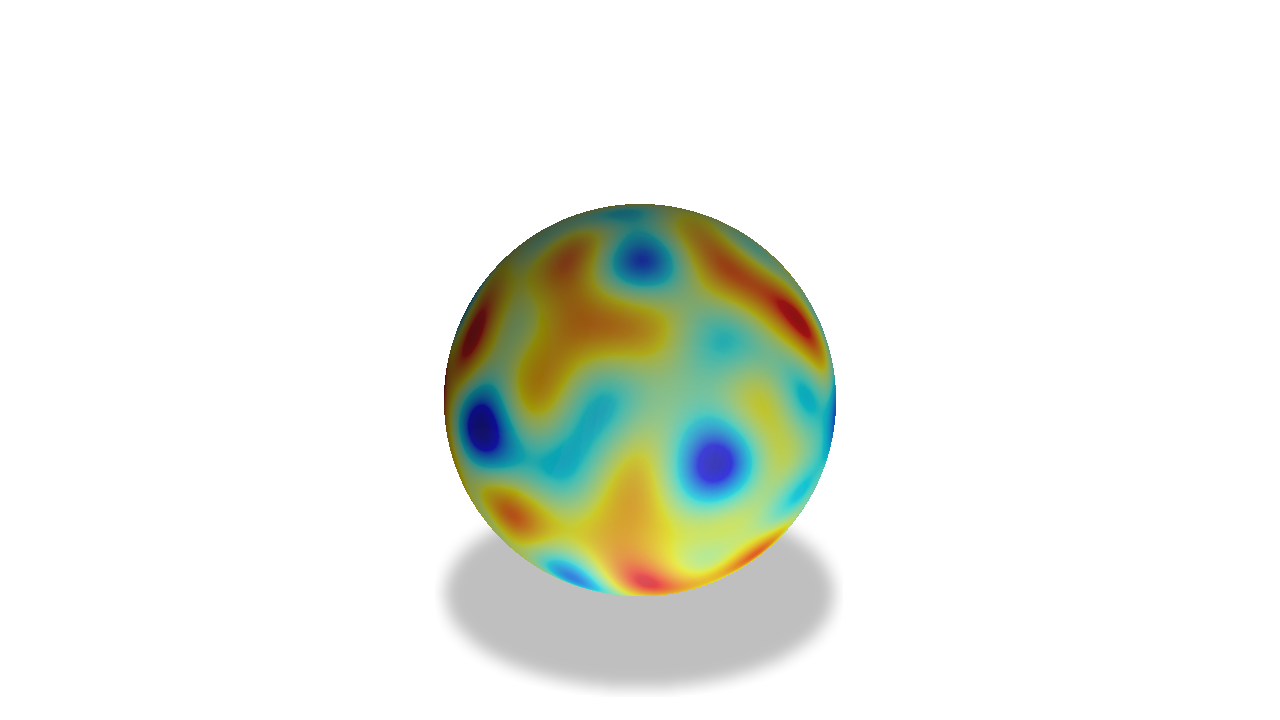
\includegraphics[clip, trim=12cm 0cm 12cm 7cm,width=\textwidth]{sphere}
  \caption{Sphere}
  \label{fig:sphere}
\end{subfigure}\hfil % <-- added
\begin{subfigure}{0.3\textwidth}
  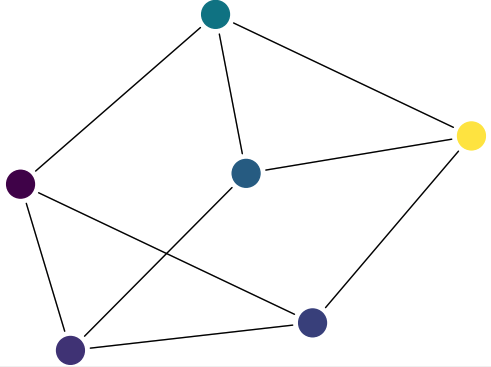
\includegraphics[clip, trim=0cm .05cm 0cm 0cm, width=\textwidth]{graph}
  \vspace{.5cm}
  \caption{Graph}
  \label{fig:graph}
\end{subfigure}\hfil % <-- added
\begin{subfigure}{0.3\textwidth}
  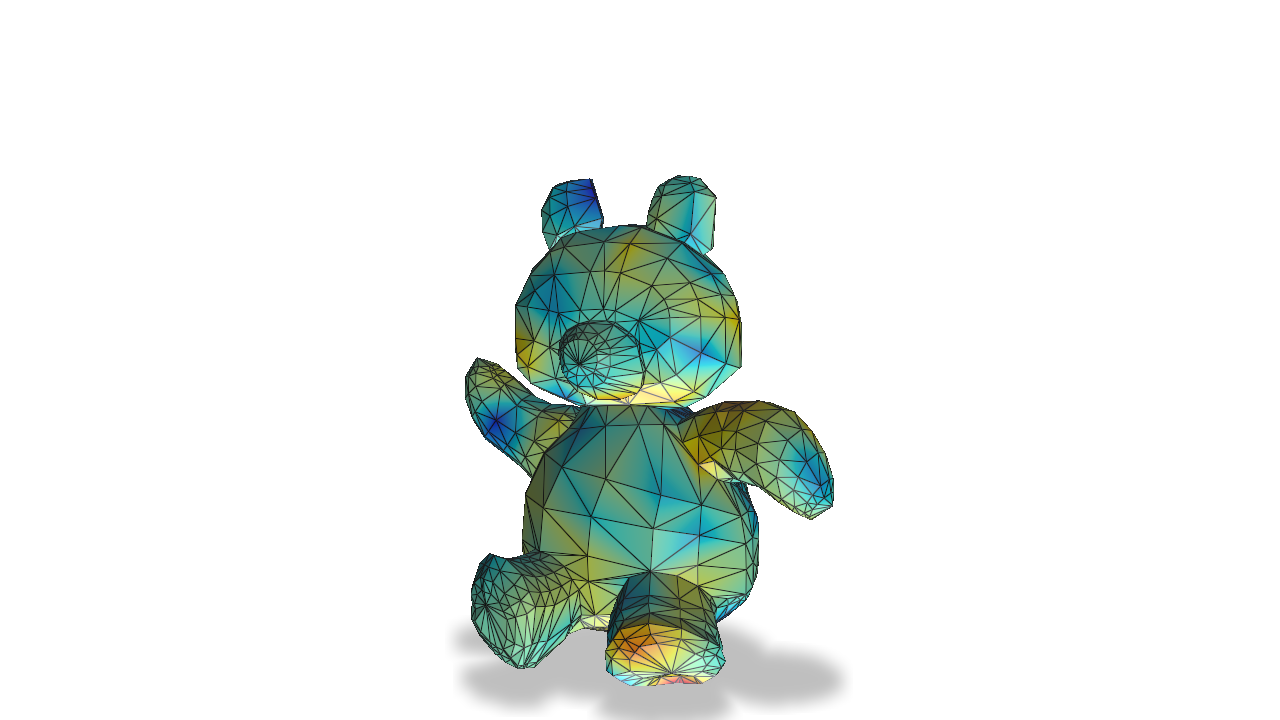
\includegraphics[clip, trim=12cm 0cm 12cm 5cm,width=\textwidth]{teddy_mesh}
  \caption{Mesh}
  \label{fig:mesh}
\end{subfigure}
\caption{Mat\'ern GP samples on non-Euclidean spaces}
\label{fig:gp-noneuclidean}
\end{figure}

Stationary kernels are ubiquitous in Gaussian processes when the input space is Euclidean. Their popularity is due to their general useability and the ease of understanding the prior information they encode. Recent work of \citet{Borovitskiy2020} has extended the definition of stationary kernels to Riemannian manifolds. This enables the definition of symmetric and positive-definite kernels, which characterise GPs, that take into account the geometry of the space. In the case of a graph, for example, two nodes can be close to each other in the Euclidean space yet far apart in the term of number of edges them separates them. A classical stationary kernel is not able to capture this information, whereas a geometric aware kernel can.

The construction in \citet{Borovitskiy2020} relies on the spectral theory of the Laplace-Beltrami operator and defines the kernel through its Mercer decomposition (\cref{eq:mercer})
\begin{equation}
    \label{eq:borovitskiy}
    k(x, x) = \sum_i S(\sqrt{\lambda_i})\,\phi_i(x)\,\phi_i(x')
\end{equation}
where $S$ is the power spectrum of the kernel and $\{\lambda_i, \phi_i\}$ are the eigenvalues and eigenfunctions of the Laplace-Beltrami operator. \cref{chapter:vish} discusses a special case of this construction for zonal kernels defined on the hypersphere where the eigenfunctions are given by the spherical harmonics.

The elegance of \cref{eq:borovitskiy} is that it defines the kernel through the eigenfunctions of the Laplace-Beltrami operator. These eigenfunctions are known analytically for certain well-studied manifolds, such as the sphere and the torus. However, in practice, working with more complex manifolds involves discretising the manifold of which the mesh and undirected weighted graph are special cases. This unifying theory allows us to directly define kernels on these spaces, as illustrated by \cref{fig:gp-noneuclidean}.

Given the brief background on model-based approaches to MDP and Gaussian processes defined on non-Euclidean spaces we now suggest the following research agenda. 

\section{Research Agenda}
The overarching theme of my proposed research agenda is: ``How can we make Gaussian processes an effective tool for model-based decision-making on non-Euclidean spaces?''. The ultimate goal would be that these tools are more widely used outside our `small' GP community by domain experts. For instance, one could envision these tools to be particularly useful in civil engineering, where finite element meshes are commonplace; for environmental and climate modelling on a sphere to represent our globe; or for molecular design using graph structures. To achieve this goal we need at least the following components:

\subsection{Adoption: Geometric Kernel Package}

\begin{figure}
    \centering
    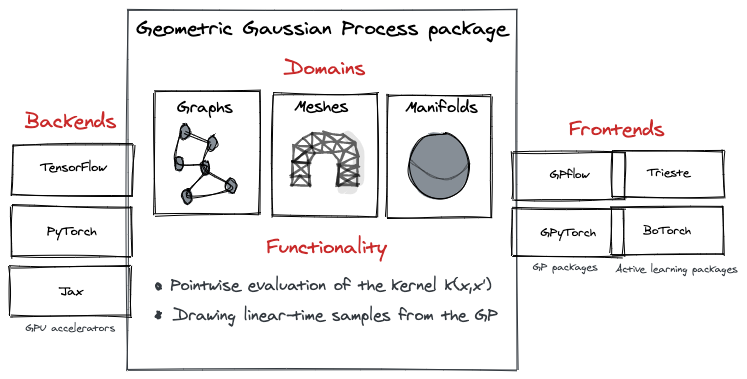
\includegraphics[width=.7\textwidth]{geomgp}
    \caption{Overview of Geometric Kernel package}
    \label{fig:geomgp}
\end{figure}

Open-source, high-quality software is a key catalyst for good research: it allows one to quickly prototype ideas on top of strong foundations, but---more importantly---it makes it possible to share ones work with the wider community. A important objective in this research agenda is to develop a Python package which provides implementations of geometric kernels defined on manifolds, meshes and graphs. We envision the package to be opinionated on the best way to handle these manifold objects. However, to not hinder adoption by the wider community we believe the package should be backend agnostic. This will enable its use in downstream GP packages in both TensorFlow (e.g., GPflow) and PyTorch (e.g., GPytorch). \Cref{fig:geomgp} gives an overview of the package. The development has started at \url{https://github.com/GPflow/GeometricKernels}.

\subsection{Efficiency: Sparse Manifold Gaussian processes}

The cubic computational complexity of GPs in Euclidean spaces limits their use in many real-world applications. As explained in \cref{chapter:theoretical-framework}, a widely adopted solution to this problem is to employ a smaller set of inducing points which summarise the GP at a set of optimised input locations. Not surprisingly, the same cubic computational complexity is present in the non-Euclidean counterpart of GPs. It is, unfortunately, not straightforward to extend the inducing point solution to these domains. For example, it is not clear how to define an inducing variable on a graph or on a mesh, and how one would freely optimise their location to minimise the KL divergence between true and approximate posterior---as is the case with traditional inducing point inputs. The interdomain and eigenfeatures inducing variable approach, introduced in \cref{chapter:theoretical-framework,chapter:vish}, seems a promising route as the resulting basisfunctions are fixed, and by construction optimally placed for a given geometry (see \cref{sec:vff-vs-vish}). The objective of this research project is to develop a scalable method for GPs on manifolds, akin to the methods that one has at their disposable in the Euclidean case. This will enable both larger dataset, as well as non-Gaussian likelihoods.

\subsection{Application: Sequential decision-making on non-Euclidean spaces}

To convince a wider audience to use these methods, it is important to show their practical usefulness on a real-world use-case. While the exact application is, at the time of writing, not set in stone, we consider the use-case of `planning searches for lost aircrafts and other objects' \citep{stone2014search} to be an well-suited problem to test our methods. In it simplest formulation, planning a search mission can be seen as a Bayesian optimisation problem, where the optimisation surface is mainly flat (i.e. absence of the aircraft), apart from a single global minimum at the location of the lost object. However, the problem quickly becomes more challenging---and realistic---when we consider observations to be noisy. This is indeed important because it is likely that the missing aircraft will have sunk, and not observing it does not necissarily mean its absence. Additionally, it will also be necessary to take into account water and wind currents, which will give a time-varying aspect to the problem. Finally, one will have to consider the cost associated to moving the search operation, which will imply a different regret compared to the traditional one used in BO (given in \cref{eq:regret-bo}). Given the geometry of our globe this is a problem that is most naturally represented on the sphere. This representation will also come in handy when visualising results and for encoding prior information into the models (e.g., flight and current models), which highlights the importance of our work on decision-making on non-Euclidean spaces.


% An interesting extension to this problem 

% Basically settings where DNNs are never going to be competitive with GPs - low-dim, very data-efficient, high-cost - not even if someone figures out how to do DNN uncertainty right, due to GP regret guarantees (under reasonable assumptions) matching the best possible regret achievable by any model/decision system.

% \paragraph{Related areas}
% \begin{enumerate}
%     \item Probabilistic numerics [Tubingen Manifesto, Osborne and Henning]. They are less interested in closing the loop and making decisions atop of the models. They usually plot the error bars on the estimator as their final result.
%     \item Bayesian optimisation methods. Special case.
% \end{enumerate}



%%% OLD:

% Through this line of work, I believe that we have showed that (deep) Gaussian processes are an interesting non-parametric alternative to Bayesian neural networks (BNNs). Our work differs from the conventional BNN literature in that we attempt to scale well-understood fully-Bayesian models (i.e. GPs) to big data settings, rather than the converse: starting from complex parametric models and trying to approximate Bayesian inference in them. The former strategy allows to gradually build up complexity into the models while maintaining their favourable properties, such as a marginal likelihood objective and good uncertainty quantifications.

% In what comes next, I want to separate the different regimes in which neural networks and Gaussian processes operate and thrive. For example, NNs can handle---and in practice require---very large datasets, whereas Gaussian process models are more comfortable in the small data regime. Neural networks, in the presence of large datasets, are extremely good at learning complex latent representations, as evidenced by the latest models in natural language processing and computer vision. Non-parametric Gaussian processes, on the contrary, work best on limited and noisy datasets. Datasets where each datapoint can be very expensive in terms of cost or time to obtain. I believe that this is a setting---in the era of deep learning---that has been under studied and valued, yet of high importance for many scientific or commercial applications.

% Many real-world problems can be described as inferring properties of an expensive black-box function $f: \mathcal{X} \rightarrow \mathcal{Y}$, subject to a computational budget of $T$ function evaluations. Typical examples are (global) optimisation, finding a level set (i.e. the set of points in $X \subset \mathcal{X}$ for which $f(x) > C,\forall x \in X$), or finding the shortest path between two nodes in a graph. In the graph example, the black-box function $f$ would return the cost of traversing an edge and query the cost of an edge would be very expensive. Naively applying Dijkstra would require the evaluation of $f$ at every edge and thus potentially grossly exceeding the given budget of $T$ evaluations.


% \begin{enumerate}
%     \item Black Box Functions $f: \mathcal{X} \rightarrow \mathcal{Y}$
%     \item We want to estimate a computable property $\mathcal{O}_\mathcal{A}(f)$
%     \item $\mathcal{A}$ is an algorithm $\mathcal{O}_\mathcal{A}(f) = \mathcal{A}(f)$
%     \item Evaluating $f$ is \emph{very} expensive (we can only evaluate it a limited amount of times)
% \end{enumerate}

% \paragraph{Examples}
% \begin{enumerate}
%     \item Optimisation: $\mathcal{A}(f) = \argmax_{x\in\mathcal{X}} f(x)$, which implies $\mathcal{O}_\mathcal{A}(f) = x^*$.
%     \item Sensor Placement (Active Learning): $\mathcal{O}_\mathcal{A}(f) = \argmax_{X \subset \mathcal{X}, |X| = T} \textrm{MI}(f, f(X))$.
%     \item Level sets: $\mathcal{O}_\mathcal{A}(f) = \{X \subset \mathcal{X}: f(x) > C, \forall x \in X\}$.
%     \item Shortest path: $\mathcal{O}_\mathcal{A}(f) = $ shortest path between two nodes in a graph.
% \end{enumerate}

% \paragraph{Real-world problems}
% \begin{itemize}
%     \item[Graphs] Social networks. Search for cliques or shortest paths.
%     \item[Meshes] Aerospace and civil engineering problems. ``General'' sensor placement.
%     \item[Manifold] Sphere. Interesting problem in astrophysics: when a gravitational wave detection is made there's usually a very large uncertainty of its origin so optical telescopes have to sweep the sky looking for the source.
% \end{itemize}

% \paragraph{Objectives}
% \begin{enumerate}
%     \item Theory and analysis
%     \item Show the excellence of Gaussian processes in this regime
%     \item Benchmarks for future methods
% \end{enumerate}